%%%%%%%%%%%%%%%%%%%%%%%%%%%%%%%%%%%%%%%%%%%%%%%%%%%%%%%%%%%%%%%%%%%%%%% SETUP %
\documentclass[journal]{IEEEtran}
\usepackage{cite}
\usepackage{amsmath,amssymb,amsfonts}
\usepackage{algorithmic}
\usepackage{graphicx}
\usepackage{textcomp}
\usepackage{xcolor}
\usepackage{rotating}
\usepackage{lscape}
\usepackage{caption}
\usepackage{listings}

\def\BibTeX{{\rm B\kern-.05em{\sc i\kern-.025em b}\kern-.08em
    T\kern-.1667em\lower.7ex\hbox{E}\kern-.125emX}}

\def\tt#1{\mbox{\texttt{#1}}}

\newcommand*{\thead}[1]{\multicolumn{1}{c}{\bfseries #1}}

\definecolor{codegreen}{rgb}{0,0.6,0}
\definecolor{codegray}{rgb}{0.5,0.5,0.5}
\definecolor{codepurple}{rgb}{0.58,0,0.82}
\definecolor{backcolour}{rgb}{0.95,0.95,0.92}

\lstdefinestyle{codestyle}{
    backgroundcolor=\color{backcolour},
    commentstyle=\color{codegreen},
    keywordstyle=\color{magenta},
    numberstyle=\tiny\color{codegray},
    stringstyle=\color{codepurple},
    basicstyle=\ttfamily\footnotesize,
    breakatwhitespace=false,
    breaklines=true,
    captionpos=b,
    keepspaces=true,
    numbers=left,
    numbersep=5pt,
    showspaces=false,
    showstringspaces=false,
    showtabs=false,
    tabsize=2,
    xleftmargin=.125in,
    xrightmargin=.0in
}
\lstset{style=codestyle}

\begin{document}


%%%%%%%%%%%%%%%%%%%%%%%%%%%%%%%%%%%%%%%%%%%%%%%%%%%%%%%%%%%%%%%%%%%%%%% TITLE %

\title{Flawfinder and Secure Development Processes}

\author{\IEEEauthorblockN{Kevin Kredit}
\IEEEauthorblockA{\textit{GVSU CIS Department} \\
Grand Rapids, Michigan \\
Email: k.kredit.us@ieee.org}
}

\maketitle


%%%%%%%%%%%%%%%%%%%%%%%%%%%%%%%%%%%%%%%%%%%%%%%%%%%%%%%%%%%%%%%%%%%%%%% ABSTRACT %

\begin{abstract}
Static analysis tools provide insights to security and correctness early in the software development
process. Flawfinder is a static analysis tool for C and C++ focusing on dangerous method use. It
performs a syntax-aware search, identifies dangerous functions uses, and prints a ranked list of
warnings. A complete secure development process may employ multiple static analysis tools. Statick
is a plugin-based framework to manage multiple tools, including Flawfinder. To simplify the workflow
for small projects, a Docker container has been built with a portable Statick environment.
\end{abstract}

\begin{IEEEkeywords}
Flawfinder, Statick, static analysis, secure software, development process
\end{IEEEkeywords}


%%%%%%%%%%%%%%%%%%%%%%%%%%%%%%%%%%%%%%%%%%%%%%%%%%%%%%%%%%%%%%%%%%%%%%% PAPER %

\section{Introduction}

Security cannot be bolted on. The sooner project developers consider security, the cheaper it is to
achieve. If a project can continuously validate application security principles before it is
finished, or even before it builds, it will experience fewer costly surprises later on.

Static analysis tools provide this continuous validation capability. They read source code and
report possible errors in a developer-friendly format. Other validation techniques such as
functional tests, unit tests, binary analysis, and runtime analysis require varying levels of
readiness. Because static analysis tools require only source code, developers can integrate them
from the beginning of the process.

Flawfinder is a static analysis tool for C and C++ \cite{flawfinder}. It works by searching for
invocations of dangerous or hard to use functions, ranking them based in order of risk, and
displaying them with helpful messages.

This paper gives a brief overview of static analysis tools in general, including their purpose,
their capabilities and limitations, and how they fit in a secure software engineering workflow. It
then describes Flawfinder in particular, including how it works, how it is configured, and example
output from running it against a real project. Finally, it strives to lower the barrier for static
analysis tool usage by describing the Statick framework and introducing a project that provides the
Statick environment in a portable Docker container.


\section{Static Analysis Tools}

Static analysis tools read source code files and produce warnings related to incorrect or dangerous
constructs. Because they do not compile or execute code, there are limitations on what types of
errors they can detect. Therefore, they comprise only a part of a complete secure software
development process.

\subsection{Capabilities}

Analyzing source code provides several capabilities.

\paragraph{Analyze during development} As already established, considering security late in the
development process is difficult and costly. A major advantage of static analysis tools is that they
do not require a complete product to test; they do not even require code to compile or contain valid
syntax. Teams can setup static analysis tools at the start of a project and reap the benefits from
the first line of code.

\paragraph{Correct little human errors} Humans make frequent trivial errors. By negligence or
ignorance, developers make typos and violate coding standards. Working with editors and compilers,
source code analysis tools can identify and correct spelling errors and enforce coding standard
rules.

\paragraph{Identify dangerous method usage} Many standard software libraries contain dangerous or
difficult to use methods. For example, the C standard library's \tt{strcpy} is highly vulnerable to
buffer overflows, and the safer \tt{strncpy} should be used instead. \tt{strcpy} cannot be removed
from the library for the sake of backwards compatibility. To prevent its use in new code, static
analysis tools can detect such usage.

\paragraph{Identify dangerous syntax idioms} Sometimes syntactic features that lead to concise code
can also lead to confusion, and confusion leads to errors. Static analysis can identify these
dangerous idioms.

\paragraph{Apply rigorous logical analysis} Beyond some of the simple applications, advanced static
analysis can detect errors that would take a human a long time to identify. Through control or data
flow analysis, it can detect dead code, memory errors, and information leakage. This type of
advanced analysis is typically computationally expensive and limited by the semantics of the
language under analysis (e.g., the rules of Rust enable stronger static guarantees than C).

\subsection{Limitations}

Analyzing source alone also entails limitations.

\paragraph{No functional testing} Source code analysis is not intelligent to tell whether code is
semantically correct. Functional tests are still necessary to ensure correct feature implementation.

\paragraph{No compiler validation} A fully verified toolchain requires certification that the
compiled assembly code correctly implements the uncompiled source. Functional testing informally
tests this; static analysis cannot.

\paragraph{No higher order logic validation} Many security vulnerabilities are the result of
insecure designs, not insecure implementations. Algorithm, protocol, and architecture analysis are
not within the scope of static analysis tools.

\subsection{Secure Software Development Process}

A complete secure software development process includes many steps in addition to static analysis.
Microsoft has developed a detailed sequence of steps called the ``Microsoft Software Development
Lifecycle'' (or SDL). The complete lifecycle is shown in figure \ref{fig:ms_sdl}.

The SDL contains five development stages: requirements, design, implementation, verification, and
release. The security focus of each stage is shown in table \ref{table:sdl_security}.

\begin{table}[h]
    \centering
    \begin{tabular}{|l|p{.3\textwidth}|}
        \hline
        \thead{Stage} & \thead{Security Aspects} \\ \hline
        Requirements &
            Security requirements; define bug tracking process
            \\ \hline
        Design &
            Consult advisors on security; minimize attack surface; perform threat modeling
            \\ \hline
        Implementation &
            Specify toolchain and flags; run static analysis; minimize bad APIs
            \\ \hline
        Verification &
            Dynamic analysis; fuzz testing; penetration testing
            \\ \hline
        Release &
            Document incident response procedure; final security review
            \\ \hline
    \end{tabular}
    \caption{Security Aspects of SDL Stages}
    \label{table:sdl_security}
\end{table}

These stages demonstrate that static analysis is only one tool among many. As Flawfinder's homepage
says, ``No tool can substitute for human thought! ... `a fool with a tool is still a fool'. It’s a
mistake to think that analysis tools (like flawfinder) are a substitute for security training and
knowledge.'' Static analysis tools supplement training, disciplined bug tracking and incident
response, threat modeling, dynamic testing, fuzz testing, penetration testing, and holistic reviews.

The SDL stages are based on the waterfall approach to software development. However, the concepts
can be applied to agile if the cycle times are compressed from project-scale to sprint-scale.

% Down here because takes whole page
\onecolumn
\begin{landscape}
\begin{figure}
    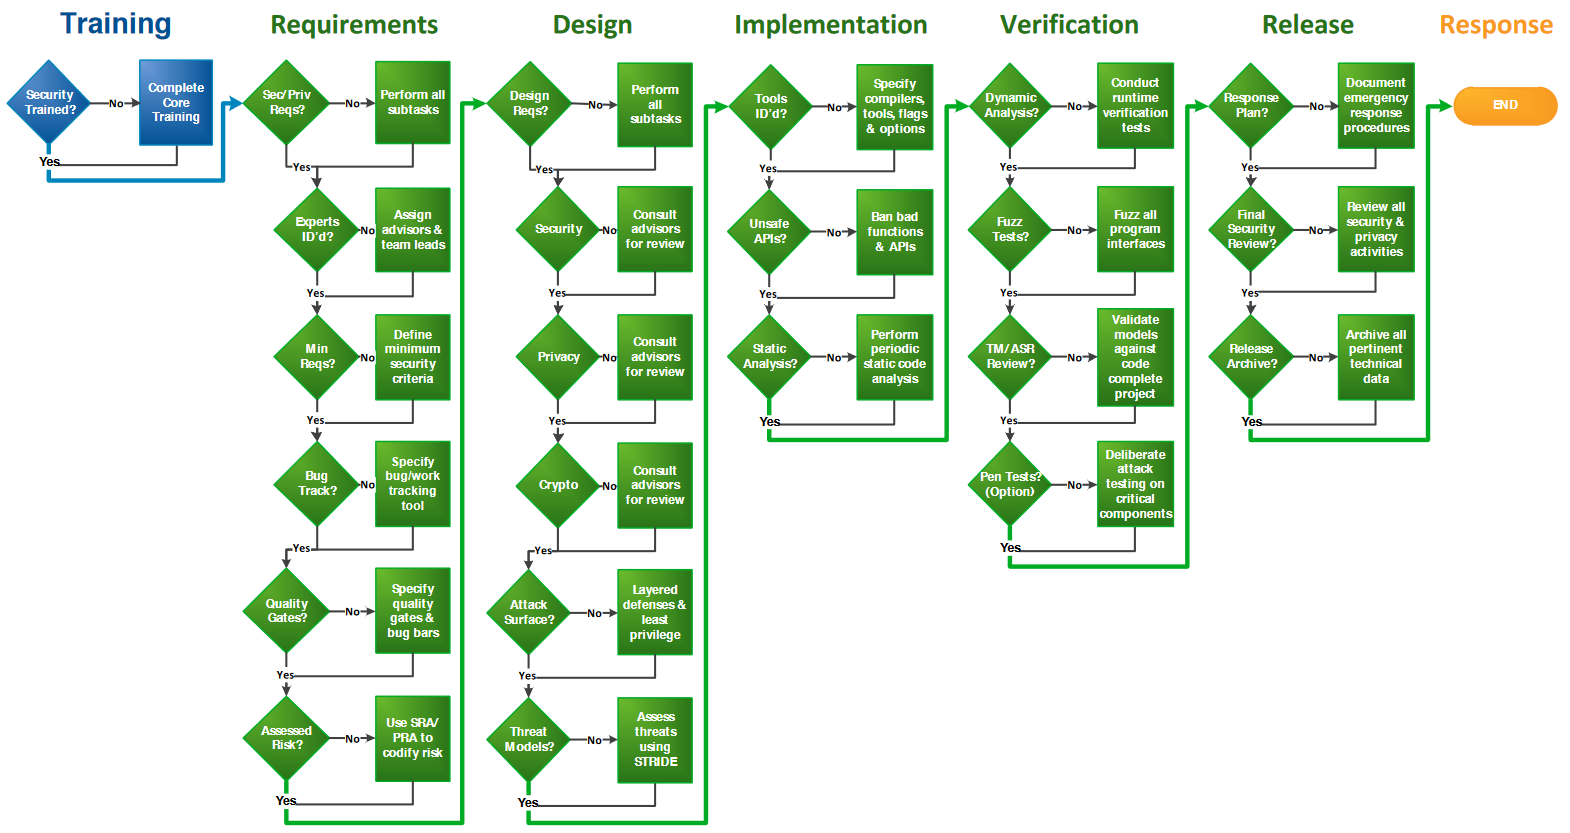
\includegraphics[width=1.0\linewidth,height=1.0\textheight,keepaspectratio]{images/microsoft_sdl_process.png}
    \captionsetup{justification=centering}
    \caption{The Microsoft Software Development Lifecycle Process \cite{ms_sdl}}
    \label{fig:ms_sdl}
\end{figure}
\end{landscape}
\twocolumn


\section{Flawfinder}

The above section discusses static analysis tools in general. This section analyzes one such tool,
Flawfinder.

\subsection{Purpose}

Flawfinder is a free and open source C/C++ static analysis tool licensed under the GNU Public
License version 2. The project is defined by simplicity. It is simple in concept, simple in
implementation, and simple to use.

Flawfinder focuses on just one of static analysis tools' capabilities listed above--to identify
dangerous method usage \cite{flawfinder}. C and C++ standard libraries contain many functions with
potential security vulnerabilities. The languages are memory unsafe and do not enforce robust error
handling. Further, they are used in many security-critical operating system settings. Flawfinder's
simple, core purpose is to identify usage of these dangerous methods, rank each instance's risk, and
present an ordered list of potential vulnerabilities to the developer. This is its entire function.

Flawfinder is also simple in implementation. Though it analyzes C and C++, it is written in Python.
Python is a more expressive language with more powerful string parsing capabilities than C or C++.
Python is not as performant as C or C++, but at 45,000 lines/second on 2014 hardware, it is as fast
as it needs to be. Lastly, Python has a mature environment of libraries and developers, which means
that the runtime is present by default on most machines and future generations can take over
development when David Wheeler, the project's main author, no longer personally maintains the
project.

Finally, Flawfinder is designed to be simple to use. It can be installed and ran using the commands
in listing \ref{lst:ff_usage}.

\begin{lstlisting}[language=sh, caption=Flawfinder Basic Usage, label=lst:ff_usage]
pip install flawfinder
flawfinder sourceFile.c
flawfinder sourceDir/
\end{lstlisting}

If Python is already installed, installing Flawfinder requires a single command, shown in line 1.
Flawfinder can be run on a single file as shown in line 2, or recursively on a directory as shown in
line 3.

\subsection{How It Works}

Flawfinder analysis runs in a basic sequence outlined in the following sections.

\subsubsection{Load a Database of Functions}

First, Flawfinder loads a database of error-prone or insecure C and C++ standard library functions.
Functions may end up in this list because they are prone to ``buffer overflow risks, format string
problems, race conditions, potential shell metacharacter dangers, and poor random number
acquisition'' \cite{flawfinder}. This database contains information on the function name, the type
of risk it poses, and the magnitude of that risk. The database itself is valuable tool in its own
right.

\subsubsection{Find Function Hits}

Second, Flawfinder searches the source code for instances of the functions in the database. This
search is somewhat smart--it doesn't do full language parsing, but it does differentiate between
code, comments and strings. This makes it smarter than a simple search tool, like \tt{grep}.
Flawfinder will also ignore hits in lines that include the comment \tt{/* Flawfinder: ignore */}.
This is so that developers can silence warnings for cases that they have analyzed and confirmed to
not be real issues.

\subsubsection{Produce a Report of Hits Sorted by Risk}

Third, Flawfinder sorts the hits according to risk and prints a report for the user. The risk and
description of the possible vulnerability are other fields in the database. The format of the report
can be set using command line arguments. The user can tune the sensitivity to false positives, set
a severity reporting threshold, and specify text formatting options.

\subsection{Example}

An example will demonstrate Flawfinder in action. Listing \ref{lst:example_code} shows a small C
program.

\begin{lstlisting}[language=c, caption=C Example Program, label=lst:example_code]
#include <stdio.h>
#include <stdlib.h>

int getNumber() {
    char numberBuffer[10];
    gets(numberBuffer);
    return atoi(numberBuffer);
}

int main() {
    printf("This program multiplies two "
           "numbers.\n");

    printf("Enter number one: ");
    int m1 = getNumber();
    printf("Enter number two: ");
    int m2 = getNumber();

    printf("\nThe product of %d and %d is %d\n",
           m1, m2, m1 * m2);

    return 0;
}
\end{lstlisting}

This program has a few obvious problems in the \tt{getNumber()} function. First, it uses a
fixed-size buffer for user input. This might not matter if the input is handled correctly, but
second, it uses \tt{gets()} to read from \tt{stdin}. \tt{gets} does not check for buffer overflows.
Third, it uses \tt{atoi} without checking for error conditions. Aside from security implications,
this program may simply crash or produce illogical results without doing more to validate the input.

Running Flawfinder on this file produces the results in listing \ref{lst:example_results}.

\begin{lstlisting}[caption=Example Flawfinder Results, label=lst:example_results]
./example.c:6:  [5] (buffer) gets:
  Does not check for buffer overflows (CWE-120, CWE-20). Use fgets() instead.
./example.c:5:  [2] (buffer) char:
  Statically-sized arrays can be improperly restricted, leading to potential
  overflows or other issues (CWE-119:CWE-120). Perform bounds checking, use
  functions that limit length, or ensure that the size is larger than the
  maximum possible length.
./example.c:7:  [2] (integer) atoi:
  Unless checked, the resulting number can exceed the expected range
  (CWE-190). If source untrusted, check both minimum and maximum, even if the
  input had no minus sign (large numbers can roll over into negative number;
  consider saving to an unsigned value if that is intended).
\end{lstlisting}

Full source for the example file and Flawfinder output is available online \cite{this_repo}.

\section{Easy Static Analysis}

\subsection{Lower the Barrier to Entry}

\subsection{Frameworks}

\subsection{Docker Container}


\section{Conclusion}
Conclusion.


%%%%%%%%%%%%%%%%%%%%%%%%%%%%%%%%%%%%%%%%%%%%%%%%%%%%%%%%%%%%%%%%%%%%%%% BIBLIOGRAPHY %

\begin{thebibliography}{00}

\bibitem{flawfinder} D. Wheeler, "Flawfinder Home Page", \textit{Dwheeler.com}, 2019. [Online].
Available: https://dwheeler.com/Flawfinder/. [Accessed: 02- Nov- 2019].

\bibitem{statick} "sscpac/statick", \textit{GitHub}, 2019. [Online]. Available:
https://github.com/sscpac/statick. [Accessed: 02- Nov- 2019].

\bibitem{ms_sdl} "Simplified Implementation of the Microsoft SDL", \textit{Microsoft.com}, 2010.
[Online]. Available: https://www.microsoft.com/en-us/download/details.aspx?id=12379. [Accessed: 13-
Nov- 2019].

\bibitem{this_repo} "kkredit/static-analysis-research-paper", \textit{GitHub}, 2019. [Online].
Available: https://github.com/kkredit/static-analysis-research-paper. [Accessed: 18- Nov- 2019].

\end{thebibliography}


\end{document}


%%%%%%%%%%%%%%%%%%%%%%%%%%%%%%%%%%%%%%%%%%%%%%%%%%%%%%%%%%%%%%%%%%%%%%% REFERENCE %

% \begin{equation}
% a+b=\gamma\label{eq}
% \end{equation}

% \paragraph{A labeled paragraph} With some text.

% \begin{table}[htbp]
% \caption{Table Type Styles}
% \begin{center}
% \begin{tabular}{|c|c|c|c|}
% \hline
% \textbf{Table}&\multicolumn{3}{|c|}{\textbf{Table Column Head}} \\
% \cline{2-4}
% \textbf{Head} & \textbf{\textit{Table column subhead}}& \textbf{\textit{Subhead}}&
%\textbf{\textit{Subhead}} \\
% \hline
% copy& More table copy$^{\mathrm{a}}$& &  \\
% \hline
% \multicolumn{4}{l}{$^{\mathrm{a}}$Sample of a Table footnote.}
% \end{tabular}
% \label{tab1}
% \end{center}
% \end{table}

% \begin{figure}[htbp]
% \centerline{\includegraphics{fig1.png}}
% \caption{Example of a figure caption.}
% \label{fig}
% \end{figure}
